\section{Connection Discovery}
\label{sec:connections}

The Vedic corpus repeats itself heavily: whole verses recur across Sa\d{m}hit\=as, and
shorter spans recur within them. Recording that as a single ``similar to'' relation
would destroy the only distinctions that make the layer usable. This section states
the algorithms, their parameters and their refusals.

\subsection{Comparison surfaces are a ladder, and it is not nested}
\label{sec:ladder}

Before any similarity is computed, a pair of texts is placed on a ladder of six
\emph{match levels}, ordered by how much a match at that level asserts:
source-exact, Unicode-normalised, punctuation-normalised, accent-insensitive,
script-folded, and sandhi-insensitive. A source-exact match says the two editions
print identical bytes; a sandhi-insensitive match says only that the two verses have
the same letters in the same order once script, accent, punctuation and word
division are all set aside. Both are real findings, they are not the same finding,
and the code states that collapsing them would be the single most misleading thing
the layer could do.

Two consequences are enforced. Which levels are \emph{reachable} depends on the
pair: a Latin-script text and a Devanagari text cannot match below script-folded, so
a report showing no source-exact matches between the \d{R}gveda and the S\=amaveda is
reporting an alphabet difference, not the absence of repetition. And the levels are
explicitly not nested, a fact relied on in thirty-five places.

\subsection{Exact parallels and variants}

\Cref{fig:crossveda} gives the counts for all four predicates by work pair.
An \emph{exact parallel} is equality on a named comparison surface, and the surface
is recorded on the edge. The live graph holds 1{,}006 such edges, and their stored
methods name the surface: script-folded (600), sandhi-insensitive, accent-insensitive
(150). A \code{VARIANT\_OF} edge (788) records a pair that matches at one level and
differs at a stronger one --- a real difference in transmission rather than a
comparison artefact.

\subsection{Near parallels: banded MinHash, then a composite score}
\label{sec:near}

Near parallels are the only layer where a genuine similarity threshold is applied,
and the corpus makes the problem tractable in a way worth stating. Over the
sandhi-insensitive surface, random-pair character-4-gram Jaccard has mean $0.006$
with a 99th percentile of $0.037$, while genuine repetitions sit above $0.45$. That
separation --- nearly two orders of magnitude --- is what makes cheap candidate
generation viable at all.

Candidate generation is banded MinHash locality-sensitive hashing over character
4-grams, with 96 permutations in 32 bands of 3 rows, using deterministic
permutations derived from a fixed seed. Buckets larger than 800 members are dropped
and the drop is reported. Scoring is then a composite over the same surface:
\[
  \mathrm{sim}(a,b) \;=\; w_{g}\,J\!\left(G_4(a), G_4(b)\right) \;+\;
                          w_{l}\,\frac{\mathrm{LCS}(a,b)}{\max(|a|,|b|)},
  \qquad w_{g}=w_{l}=0.5,
\]
where $G_4$ is the set of character 4-grams and $J$ is Jaccard. Because both terms
are bounded by $1$ and equally weighted, a pair cannot reach the floor unless each
term separately exceeds a derived bound, and those bounds are computed from the
floor rather than tuned --- applying them before the expensive \mbox{LCS} is a pure
speed-up with no recall cost.

The floor is $0.72$, with $0.85$ marking a strong match. The floor's justification
is measured rather than asserted: at $0.60$ the \d{R}gveda/Atharvaveda candidate set
is dominated by pairs sharing nothing but \iast{indra}, \iast{soma} and a case
ending. The banding is tuned so that every pair at $0.44$ or better is proposed.

\subsection{Caps are part of the contract}
\label{sec:caps}

All-pairs over 20{,}210 mantras is 204 million unordered pairs --- 408 million
ordered --- and every stage in this layer would emit a hundred million edges if
asked.\footnote{The repository's own comment says ``204 million ordered pairs'';
$\binom{20210}{2}=204{,}211{,}945$ is the unordered count, and we state the
corrected term here.} The module that holds the
caps states the governing idea: an unbounded graph is not a more complete graph, but
one in which nothing is findable and the true repetitions are buried under noise
that looks exactly like them. Three rules apply to every cap:

\begin{enumerate}[leftmargin=1.9em,itemsep=1pt,topsep=2pt]
\item \textbf{A cap that fires is reported.} A silently truncated result set is
indistinguishable from a small one.
\item \textbf{Top-$K$ beats a threshold sweep,} because it bounds the graph by
construction at a size independent of how similar the corpus happens to be. Near
parallels are capped at 5 per mantra per Veda, and the layer at 40{,}000 edges.
\item \textbf{A cap is not a quality filter.} Anything a cap drops is dropped for
being \emph{numerous}, not for being wrong, and the drop count is the honest measure
of what the layer is not showing.
\end{enumerate}

\begin{figure}[tbp]
\centering
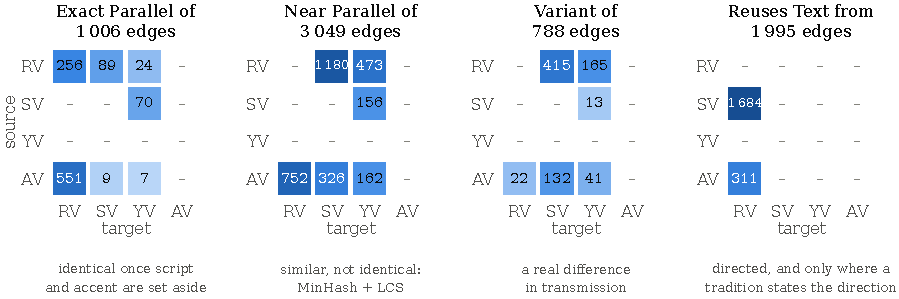
\includegraphics[width=\linewidth]{figures/fig_crossveda.pdf}
\caption{Cross-textual relationships between the four Samhit\=as, one matrix per
predicate on a shared log-scaled ramp. They are shown separately because the four
predicates assert different things; a single summed ``similarity'' matrix is the one
chart this layer exists to avoid. A dash is a measured zero, not missing data. Only
\code{REUSES\_TEXT\_FROM} is directed, and only where the direction is evidenced
(\cref{sec:reuse}).}
\label{fig:crossveda}
\end{figure}

\subsection{Formulae}
\label{sec:formula}

A \emph{formula} is a repeated multi-word span, reified as a node so that $n$
passages sharing it cost $n$ edges rather than $\binom{n}{2}$. The graph holds
4{,}825 formulae in 720 families, with 22{,}686 occurrence edges. Five bounds
control what counts, each with a stated reason:

\begin{itemize}[leftmargin=1.9em,itemsep=1pt,topsep=2pt]
\item \textbf{2 to 8 words.} One word is a lexeme --- the lemma layer already has it,
and \iast{agni} is not a formula. Above eight words a repeated span is a whole verse,
which the parallel layer already records.
\item \textbf{At least 3 distinct mantras.} Two occurrences is as often a coincidence
of sandhi as a formula.
\item \textbf{At least 12 characters.} Two very short words fold to a handful of
letters and match everywhere.
\item \textbf{At most 8\,\% of a Veda.} A span occurring in more than that share is
that Veda's grammar, not its phraseology --- and the share is computed \emph{per
Veda}, so a S\=amavedic refrain is judged against the S\=amaveda rather than against
the corpus.
\item \textbf{Ceilings} of 6{,}000 formula nodes and 120{,}000 occurrence edges, the
first because the node exists precisely to replace combinatorial edges with a hub,
and a hundred thousand hubs would defeat that.
\end{itemize}

Occurrence detection runs at two grains, and the edges record which: word-aligned
matching (20{,}577 edges) and a sandhi-insensitive substring fallback (2{,}109).
Family membership is likewise two mechanisms kept apart on the edge --- a core
grouping (1{,}828), expansion by containment (2{,}238), and a small
similarity-based extension (8) --- because the tier of a membership edge depends on
which derivation produced it, and the two directions of the mirror must be
byte-identical or a query would get a different tier depending on which way it
walked.

Contamination is a named hazard rather than an assumed absence: a documented
baseline finding records that formula nesting inflates roughly a third of
formula-bearing passages, and the containment relation is modelled explicitly so
that nesting is visible instead of double-counted.

\subsection{Ritual and material culture}
\label{sec:ritual}

The ritual layer is small but it is the clearest case in the graph for typing at the
edge rather than at the predicate, so we report it here rather than in an appendix.

The objects are modelled as distinct kinds rather than as one ``thing'' class:
103 rites, 3{,}121 ritual steps, 20 ritual roles, 21 offerings, 33 substances, 41
implements, and small populations of plants (22), animals (15), metals (7), weapons
(5) and crops (5). The step layer is the large one, and it is source-explicit: a
rite's procedural steps are what a source prints, and all 3{,}121 carry that layer.
An earlier pass had filed those steps under a generic ``Other'' category, which is a
reminder that a fine-grained vocabulary is worth nothing if the loader does not use
it.

The instructive part is the relationships. Consider two predicates:

\begin{center}\small
\begin{tabular}{@{}lrr@{}}
\toprule
Predicate & \Ltwo{} or \Lone{} & \Lfour{} \\
\midrule
\code{USED\_FOR\_RITE} & 110 & 419 \\
\code{PERFORMED\_BY}   &  16 &  16 \\
\bottomrule
\end{tabular}
\end{center}

\noindent Each carries claims of two different epistemic kinds under one name. Some
uses of a verse in a rite are derivable from what a source states about the book the
verse sits in; others are this project's reading of what the verse is for. Some
statements of who performs a rite are source-stated; an equal number are inferred.
A grade attached to the \emph{predicate} would be wrong for one population in each
row --- which is exactly the defect \cref{sec:model} describes, caught here before
it shipped rather than after.

The layer also contains the graph's only model-extracted ritual claims: 11
offering involvements, 9 ritual involvements and 3 substance involvements, 23 edges
in total, all at \Lthree{} and all excluded by a single predicate from any count a
reader wants to keep source-grounded.

Two precision controls are worth naming. Rejected candidates are retained with
reasons rather than deleted, so the offering layer ships alongside a file of
refusals. And the layer's own precision was sampled rather than assumed: a derived
metric records two figures for the ritual-context assignment --- 0.79 over every
reviewed row and 0.95 over the reproducible ones --- with a note explaining that a
single figure would have to decide whether an unreproducible row is an error or an
unknown, and that it is an unknown. That node also carries
\code{is\_human\_gold = false} and a reviewer field naming an agent, which is how
the graph says that its own quality figure is not human-adjudicated either.

\subsection{Audio, briefly}
\label{sec:audio}

Recitation audio is referenced rather than held: there is no recording node type in
the graph, and the media are linked, not mirrored. We mention the layer only because
its history contains the cleanest instance of a defect this paper's method is meant
to catch. An earlier source published one file per hymn and renumbered one
\d{R}gvedic book after a different edition's arrangement, so a key-for-key mapping
attached the wrong recitation to 55 hymns --- not a gap but a silent misalignment,
which the project's own decision record calls the worse of the two. The replacement
source was verified per verse against the stored text, and the verses it could not
verify were refused rather than mapped approximately. A separate owner decision then
made human audible review a \emph{badge} rather than a visibility gate, on the
reasoning that automated checking is not listening; the number of recordings a named
person has actually played remains small and is recorded as such.

\subsection{Direction: compilation asymmetry}
\label{sec:reuse}

Identifying that two verses are parallel says nothing about which way the borrowing
ran. The project initially asserted direction for exactly one pair --- 1{,}684
S\=amaveda-to-\d{R}gveda edges --- on a \emph{tradition's} statement that the
\=Arcika is a collection of \d{R}gvedic verses arranged for chanting, and left every
other pair undirected on the ground that asserting a direction there would be a
chronology claim. The weakness was that all 1{,}684 edges carried the identical
justification sentence: a pipeline constant that says why the class is directed and
nothing about the edge it sits on.

The replacement is a measured, per-edge signal. A borrowed verse and its source are
by construction nearly identical, so nothing about the strings can point. What points
is the company each verse keeps. A compiler assembles a unit out of verses drawn from
elsewhere, so its unit is largely made of counterparts, and those counterparts are
scattered across many units of the other corpus; a composer's hymn is not made of
anything, and only some of its verses happen to have been taken. For each side,
measured on that side's own containing unit:
\[
  \text{share} = \frac{|\{v \in U : v \text{ has a counterpart}\}|}{|U|},
  \qquad
  \text{dispersion} = |\{\,U' : \text{some counterpart lies in } U'\}|.
\]
Direction is asserted from the high-share side to the low-share side, and only when
share $\ge 0.5$ and the margin between sides is $\ge 0.25$.

Two preconditions refuse pairs before the measure runs, both on measured grounds.
\emph{\d{R}gvedic mediation}: if two verses in different corpora are both
counterparts of the same \d{R}gvedic verse, those corpora share \d{R}gvedic text
rather than each other's --- measured at 96.1\,\% of Atharvaveda/S\=amaveda pairs,
95.4\,\% of S\=amaveda/Yajurveda and 83.3\,\% of Atharvaveda/Yajurveda, against
0.0\,\% of \d{R}gveda/Yajurveda. \emph{Unit granularity}: the measure is a ratio over
a structural unit, and the median containing unit holds 9 verses in the \d{R}gveda,
4 in the Atharvaveda, 3 in the S\=amaveda --- and 44 in the Yajurveda, whose smallest
container here is the \iast{adhy\=aya}. A share over a 44-verse unit is not the same
instrument as a share over the three-verse unit that is modal in the S\=amaveda
(281 of its 458 containing units hold exactly three verses, whatever the addressing
calls them), so every Yajurvedic pair is
refused.

Finally the instrument is only allowed to speak in a scope where it demonstrates
both power (at least 100 directed verdicts) and internal consistency (at least
90\,\% pointing the same way). The scope table is the interesting output:

\begin{center}\small
\begin{tabular}{@{}lrrl@{}}
\toprule
Scope & Directed & Consistency & Outcome \\
\midrule
\d{R}gveda/S\=amaveda, whole pair & 1{,}212 & 0.991 & accepted, SV $\to$ RV \\
Atharvaveda/\d{R}gveda, whole pair & 480 & 0.763 & \textbf{rejected} \\
Atharvaveda/\d{R}gveda, k\=a\d{n}\d{d}a 20 & 322 & 0.966 & accepted, AV $\to$ RV \\
\d{R}gveda/Yajurveda, whole pair & 325 & 0.532 & \textbf{rejected} \\
\bottomrule
\end{tabular}
\end{center}

\noindent The method recovers the tradition's own claim about the S\=amaveda
independently, at 0.991; it localises the Atharvavedic case to k\=a\d{n}\d{d}a 20,
which is exactly the book known to be largely \d{R}gvedic; and it declines the two
scopes where it cannot separate the sides. Four typed refusal codes record which
precondition or floor rejected a pair.

\subsection{What the corpus's structure does \emph{not} establish}

One negative result belongs here because it disciplines the whole layer. The
S\=amaveda has the highest undirected parallel coverage of the four works held
here, at 1{,}677 of 1{,}844 verses --- 90.9\,\%, against 34.8\,\% for the
next-placed Yajurveda --- and that figure is routinely read as self-evident
confirmation that the S\=amaveda borrows. Against a degree-preserving permutation
null over 400 draws, \d{R}gveda/S\=amaveda containment is $6.69\times$ observed
against $5.72\times$ expected from corpus size alone: an excess of only $1.17\times$.
The recorded conclusion is that no size-independent structural signature in anything
the project holds distinguishes borrower from source for any pair --- which is
precisely why direction had to come from compilation asymmetry and from a tradition's
explicit statement, rather than from coverage.

The same audit exposed a typing defect of the kind \cref{sec:model} describes: the
parallel edges carry an evidence surface of \code{SANSKRIT}, which is true of the
pairing and false of the direction. The pairing is derived from the Sanskrit; the
direction is not.

% generated by figures-src/make_tables.py -- do not edit
\begin{table}[tb]
\centering
\caption{Cross-textual relationships between mantras, by predicate and work pair.
The four predicates are deliberately not collapsed into one ``similar to'': they
assert different things, and the strongest, \code{REUSES\_TEXT\_FROM}, is directed only
where a tradition states the direction (\cref{sec:reuse}). Pairs are shown as
source~$\to$~target.}
\label{tab:reuse}
\small
\begin{tabularx}{\linewidth}{@{}lr>{\raggedright\arraybackslash}X@{}}
\toprule
Predicate & Edges & By work pair \\
\midrule
\code{EXACT\_PARALLEL\_OF} & 1{,}006 & \footnotesize AV$\to$RV~551, RV$\to$RV~256, RV$\to$SV~89, SV$\to$YV~70, RV$\to$YV~24, AV$\to$SV~9, AV$\to$YV~7 \\
\code{NEAR\_PARALLEL\_OF} & 3{,}049 & \footnotesize RV$\to$SV~1{,}180, AV$\to$RV~752, RV$\to$YV~473, AV$\to$SV~326, AV$\to$YV~162, SV$\to$YV~156 \\
\code{VARIANT\_OF} & 788 & \footnotesize RV$\to$SV~415, RV$\to$YV~165, AV$\to$SV~132, AV$\to$YV~41, AV$\to$RV~22, SV$\to$YV~13 \\
\code{REUSES\_TEXT\_FROM} & 1{,}995 & \footnotesize SV$\to$RV~1{,}684, AV$\to$RV~311 \\
\bottomrule
\end{tabularx}
\end{table}


\subsection{A refused layer}

For completeness: a semantic-resemblance layer was proposed and refused before
import, on a re-implemented lexical control it could not beat
(\cref{sec:eval-baseline}). Zero assertions were written. Its absence from
\cref{tab:reuse} is a decision, not an omission.
